\section{Common Intermediate Language}
\label{sec:TheIntermediateLanguage}
The Common Intermediate Language (CIL) has already been mentioned briefly in the sections before, but this section will describe the IL in more detail.
All the languages targeting the \dotNET Framework compile to this CIL (see \autoref{fig:Overview_of_the_Common_Language_Infrastructure}).

\begin{figure}
  \centering
  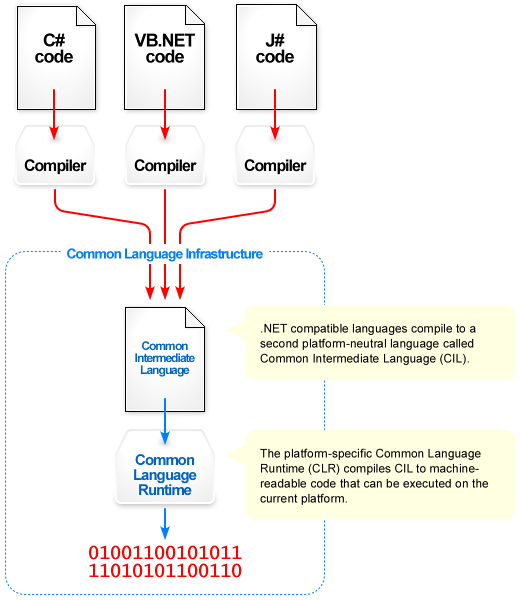
\includegraphics[style=halfheight]{Overview_of_the_Common_Language_Infrastructure}
  \caption{From source code to machine code}
  \label{fig:Overview_of_the_Common_Language_Infrastructure}
\end{figure}

A \dotNET compiler generates a \emph{managed module} which is an executable designed to be run by the CLR~\cite{Prosise2002}.
There are four main elements inside a managed module:

\begin{itemize}[noitemsep]
  \item A Windows Portable Executable (PE) file header;
  \item A CLR header containing important information about the module, such as the location of its CIL and metadata;
  \item Metadata describing everything inside the module and its external dependencies;
  \item The CIL instructions generated from the source code.
\end{itemize}

The Portable Executable file header allows the user to start the executable.
This small piece of code will initiate the just-in-time compiler which compiles the CIL instructions to native code when needed, while using the metadata for extra information about the program.
This native code is machine dependent while the original IL code is still machine independent.
This way the same IL code can be JIT-compiled and executed on any supported architecture.
The CLR cannot use the managed module directly but needs an assembly. 

An assembly is the fundamental unit of security, versioning, and deployment in the \dotNET Framework and is a collection of one or more files grouped together to form a logical unit~\cite{Prosise2002}.
Besides managed modules inside an assembly, it is also possible to include resources like images or text.
A manifest file is contained in the assembly describing not only the name, culture and version of the assembly but also the references to other files in the assembly and security requests.

\nomenclature{OpCode}{Operation Code}%
The CIL is an object oriented assembly language with around 100 different instructions called OpCodes.
It is stack-based, meaning objects are placed on an evaluation stack before the execution of an operation, and when applicable, the result can be found on the  stack after the operation.
For instance, when adding two numbers, first those numbers have to be placed onto the stack, second the add operation is called and finally the result can be retrieved from the stack.

\begin{lstlisting}[language=CIL,style=listing,caption={Adding example in IL code},label={lst:ilexample}]
.assembly AddExample {}

.method static public void main() il managed
{
  .entrypoint           // entry point of the application
  .maxstack 2

  ldc.i4 3              // Place a 32-bit (i4) 3 onto the stack
  ldc.i4 7              // Place a 32-bit (i4) 7 onto the stack
	
  add                   // Add the two and 
	                      // leave the sum on the stack
  
  // Call static System.Console.Writeline function
  // (function pops integer from the stack)
  call void [mscorlib]System.Console::WriteLine(int32)

  ret
}
\end{lstlisting}

To illustrate how to create a \dotNET program in IL code we use the previous example of adding two numbers and show the result.
In \autoref{lst:ilexample} a new assembly is created with the name \lstinline|AddExample|.
In this assembly a function \lstinline|main| is declared as the starting point (\lstinline|entrypoint|) of this assembly.
The \lstinline|maxstack| command indicates there can be a maximum of two objects on the stack and this is enough for the example method.
Next, the values 3 and 7 are placed onto the stack. The \lstinline|add| operation is called and the results stays on the stack.
The method \lstinline|WriteLine| from the \dotNET Framework Class Library is called.
This method resides inside the \lstinline|Console| class placed in the \lstinline|System| assembly.
It expects one parameter with a \lstinline|int32| as its type that will be retrieved from the stack.
The \lstinline|call| operation will transfer the control flow to this method passing along the parameters as objects on the stack.
The \lstinline|WriteLine| method does not return a value.
The \lstinline|ret| operation returns the control flow from the main method to the calling method, in this case the runtime.
This will exit the program.

To be able to run this example, we need to compile the IL code to bytecode where each OpCode is represented as one byte.
To compile this example, save it as a text file and run the \emph{ILASM} compiler with as parameter the filename.
This will produce an executable runnable on all the platforms where the \dotNET Framework is installed.

This example was written directly in IL code, but we could have used a higher level language such as C\# or VB\dotNET. For instance, the same example in C\# code is shown in~\autoref{lst:CSharpAddExample} and the VB\dotNET version is listed in~\autoref{lst:VBAddExample}. When this code is compiled to IL, it will look like the code in~\autoref{lst:ilexample}.

\begin{lstlisting}[language={[Sharp]C},style=listing,caption={Adding example in the C\# language},label={lst:CSharpAddExample}]
public static void main()
{
      Console.WriteLine((int) (3 + 7));
} 
\end{lstlisting} 

\begin{lstlisting}[language={[Visual]{Basic}},style=listing,caption={Adding example in the VB\dotNET language},label={lst:VBAddExample}]
Public Shared Sub main()
      Console.WriteLine(CType((3 + 7), Integer))
End Sub
\end{lstlisting} 

 
